\documentclass[a4paper,12pt]{article}
\usepackage[utf8]{inputenc}
\usepackage[T2A]{fontenc}
\usepackage[russian,english]{babel}
\linespread{1.5}
\usepackage{amsmath}
\usepackage{cmap}
\usepackage{booktabs}
\usepackage{caption}
\usepackage{enumitem}
\usepackage{listings}
\usepackage{xcolor}
\usepackage{setspace}
\usepackage{graphicx}
\usepackage[left=3cm, right=1cm, top=2cm, bottom=2cm]{geometry}
\renewcommand{\labelenumii}{\arabic{enumi}.\arabic{enumii}.}
\lstset{
    language=C++,
    basicstyle=\small\ttfamily,
    keywordstyle=\color{blue},
    commentstyle=\color{green!40!black},
    stringstyle=\color{purple},
    numbers=left,
    numberstyle=\tiny,
    numbersep=5pt,
    breaklines=true,
    frame=single,
    backgroundcolor=\color{gray!10},
    rulecolor=\color{black!30},
    showstringspaces=false,
    extendedchars=\true,
}
\begin{document}

\renewcommand\contentsname{Содержание}
\renewcommand{\arraystretch}{1.3} 
\thispagestyle{empty}
\begin{center}
    ФЕДЕРАЛЬНОЕ ГОСУДАРСТВЕННОЕ АВТОНОМНОЕ ОБРАЗОВАТЕЛЬНОЕ
    УЧРЕЖДЕНИЕ ВЫСШЕГО ОБРАЗОВАНИЯ
    \vspace{0.1cm}

    «КАЗАНСКИЙ (ПРИВОЛЖСКИЙ)  ФЕДЕРАЛЬНЫЙ УНИВЕРСИТЕТ»
    \vspace{0.1cm}

    ИНСТИТУТ ВЫЧИСЛИТЕЛЬНОЙ МАТЕМАТИКИ И ИНФОРМАЦИОННЫХ ТЕХНОЛОГИЙ

    Кафедра прикладной математики и искусственного интеллекта

    Направление подготовки - «Прикладная математика»
\end{center}
\vspace{2cm}

\begin{center}
    КУРСОВАЯ РАБОТА
    \vspace{0.2cm}
 
    по дисциплине: «Численные методы»
    \vspace{0.2cm}
 
    Система типа хищник-жертва. Модель Вольтерра.
\end{center}

\vfill
\vspace{3cm}
\noindent Студент 2 курса\\
группы 09-221\\
«\underline{\qquad}» \underline{\qquad\qquad} 2024 г. \qquad\qquad\quad \underline{\qquad\qquad\qquad\quad} \qquad М.А. Саитов\\
Научный руководитель\\
ассистент б.с.\\
«\underline{\qquad}» \underline{\qquad\qquad} 2024 г. \qquad\qquad\quad \underline{\qquad\qquad\qquad\quad} \qquad О.В. Глазырина
\\
\\
\\
\begin{center} \large{Казань, 2024 год} \end{center}
\thispagestyle{empty}
 

\newpage
\begin{center}
\renewcommand{\contentsname}{Содержание}
\fontsize{14}{1.15}\selectfont
\mdseries\selectfont{\tableofcontents}
\newpage
\end{center}
\setlength{\parindent}{1.25cm}
\newpage

\section{Цель работы}
\hspace{0.5cm} Целью работы является исследование модели взаимодейстия <<Хищник --- Жертва>>,
выявление зависимостей поведения модели в зависимости от значения параметров,
описывающих систему, а так же применение метода Рунге-Кутты при решении сопутсвующих систем дифференциальных 
уравнений.
\section{Теоретические основы выполнения работы}
\hspace{0.5cm} Модель Вольтерра используется для представления взаимодейстия двух типов. 
При моделировании системы <<Хищник --- Жертва>> будем учиывать следующие ограничения:
\begin{enumerate}
    \item Жертва может найти достаточно пищи для пропитания
    \item При каждой встрече с хищником последний убивает жертву
    \item Норма рождаемости жертв $x_b$, нормы естественной смертности жертв $x_d$ и\\
    хищников $c$ являются постоянными, $a = x_b - x_d > 0$.
    \item Число случаев, когда хищник убивает жертву, зависит от вероятности их
    встречи и, следовательно, пропорционально произведению $xy$. \\
    В результате встреч с жертвами число хищников увеличивается.
\end{enumerate}

Обозначим количества хищников и жертв в момент времени t через $y = y(t)$ и $x = x(t)$
соответственно. Тогда с учетом сделанных допущений, модель можно записать в виде:
\begin{equation}
    \frac{dx}{dt} = ax - bxy $$ $$
    \frac{dy}{dt} = -cy + dxy
\end{equation}
где коэффициенты $b, d$ - коэффициенты убийства жертв и воспроизводства хищников,
$a$ - описывает рождаемость жертв, $c$ - ествестенную смерть жертв. \\
Произведя в системе (1) замены:
\begin{equation*}
    X = \left(\frac{d}{a}\right)x, \hspace{0.2cm} Y = \left(\frac{b}{a}\right)y, \hspace{0.2cm} \tau = at, \hspace{0.2cm} \sigma = \frac{c}{a}
\end{equation*}
уравнение (1) преобразуется к виду:
\newpage
\begin{equation}
    \frac{dX}{d\tau} = X - XY $$ $$
    \frac{dY}{d\tau} = -\sigma Y + XY
\end{equation}
с начальными условиями:
\begin{equation}
    X(0) = X_0, \hspace{0.2cm} Y(0) = Y_0
\end{equation}
описывающими количество особей каждого из вида.
\newpage

\section{Метод Рунге-Кутты}
\hspace{0.5cm} Для решения систем дифференциалных уравнений будем использовать
метод Рунге -- Кутты 4-го порядка точности:
\begin{align}
    k_1 &= f(t_n, y_n), \nonumber \\
    k_2 &= f(t_n + \frac{h}{3}, y_n + \frac{hk_1}{3}), \nonumber \\
    k_3 &= f(t_n + \frac{2h}{3}, y_n - \frac{hk_1}{3} + hk_2),\\
    k_4 &= f(t_n + h, y_n + h(k_1 - k_2 + k_3)), \nonumber \\
    y_{n+1} &= y_n + \frac{h(k_1 + 3k_2 + 3k_3+ k_4)}{8} \nonumber
\end{align}
где $y'(t,y) = k(t,y)$. Задано начльное условие $y(0) = y_0$. Этот метод является методом
с постоянным шагом $h$ на отрезке $[a, b]$, значения решения вычисляются в $n = \frac{b-a}{h}$ точках.

Используя приведенный выше метод решить тестовую задачу:
\begin{equation}
    y'_1 = \frac{y_1}{2 + 2t} - 2ty_2, \hspace{0.5cm} y'_2 = \frac{y_2}{2 + 2t} + 2ty_1,
\end{equation}
на отрезке [0, 2].

\newpage
\section{Задание}
\hspace{0.5cm} В ходе выполнения работы необходимо:
\begin{enumerate}
    \item Проверить правильность вывода исходных уравнений (1), уравнений \\
    в безразмерном виде (2) и тестового решения (5)
    \item Найти стационарные решения (состояния равновесия) системы (2).
    \item Написать процедуру инетгрирования задачи Коши для системы из $n$ \\
    обыкновенных дифференциальных уравнений по формулам (4) на произвольном отрезке
    $[a, b]$ с постоянным шагом $h$.
    \item Для тестовой задачи (5) построить графики зависимости максимальной\\
    погрешности решения $e$ и $\frac{e}{h^4}$ от выбранного шага $h$. \\
    Пояснить результаты расчетов.
    \item Для двух наборов начальных условий (3) в окрестности состояния равновесия и нескольких значений
    параметра $\sigma$ расчитать динамику популяции. Привести графики наиболее характерных решений в координатах $(X, Z)$ и дать их \\
    интерпретацию.
\end{enumerate}
\newpage

\section{Проверка правильности вывода исходных уравнений}
\hspace{0.5cm} Для перехода от уравнения системы (1) к уравнению системы (2) мы введем новые переменные и новые параметры,
а затем проведем соответствующие замены и преобразования.

Введем следующие замены: 
\begin{equation*}
    X = \left(\frac{d}{a}\right)x, \hspace{0.3cm} Y = \left(\frac{b}{a}\right)y, \hspace{0.3cm} \tau = at, \hspace{0.3cm} \sigma = \frac{c}{a}
\end{equation*}
\hspace{0.5cm} Пойдем методом от обратного и выведем уравнения системы (1) через уравнения системы (2):
\begin{enumerate}
    \item Подставим в левую часть первого уравнения (2) наши замены получим:
    \[ \frac{dX}{d\tau} = \frac{d\left(\frac{d}{a}\right)x}{d(at)} = \frac{d}{a^2} \frac{dx}{dt} \]
    \item Подставим в правую часть наши замены получим: 
    \[ X - XY = \left(\frac{d}{a}\right)x - \left(1 - \left(\frac{b}{a}\right)y\right) \]
    \item Соединив два уравения получим:
    \[ \frac{d}{a^2} \frac{dx}{dt} = \left(\frac{d}{a}\right)x - \left(1 - \left(\frac{b}{a}\right)y\right) \]
    \item Разделив обе части уравнения на $\frac{d}{a^2}$ получим:
    \[ \frac{dx}{dt} = ax - bxy \]
\end{enumerate}

Проделав те же самые шаги ко второму уравнению системы (2), мы придем ко второму уравнению системы (1).

\newpage
\section{Решение тестовой задачи}
\hspace{0.5cm} Тестовый вариант задачи будет решен методом Рунге - Кутты 4-го порядка точности.
Дана система уравнений (5) с известным точным решением:
\begin{equation}
    y_1 = \cos(t^2)\sqrt{1 + t}, \hspace{0.5cm} y_2 = \sin(t^2)\sqrt{1 + t}
\end{equation}

Необходимо решить систему с начальными условиями $y_1(0) = 0, y_2(0) = 1$ на отрезке [0; 2].
Перед вычислением коэффициентов стоит заметить, что $y'_1 = y'_1(y_1, y_2, t)$ и $y'_2 = y'_2(y_1, y_2, t)$,
тогда:
\begin{align}
    &k_{11} = y'_1(t(i), y_1(i), y_2(i)) \nonumber \\
    &k_{12} = y'_2(t(i), y_1(i), y_2(i)) \nonumber \\
    &k_{21} = y'_1(t(i) + \frac{h}{3}, y_1(i) + \frac{h}{3}k_{11}, y_2(i) + \frac{h}{3} k_{12}) \nonumber \\
    &k_{22} = y'_2(t(i) + \frac{h}{3}, y_1(i) + \frac{h}{3}k_{11}, y_2(i) + \frac{h}{3} k_{12}) \nonumber \\
    &k_{31} = y'_1(t(i) + \frac{2h}{3}, y_1(i) - \frac{h}{3}k_{11} + hk_{21}, y_2(i) - \frac{h}{3}k_{12} + hk_{22}) \\
    &k_{32} = y'_2(t(i) + \frac{2h}{3}, y_1(i) - \frac{h}{3}k_{11} + hk_{21}, y_2(i) - \frac{h}{3}k_{12} + hk_{22}) \nonumber \\
    &k_{41} = y'_1(t[i] + h, y_1(i) + h (k_{11} - k_{21} + k_{31}), y_2(i) + h(k_{12} - k_{22} + k_{32})) \nonumber \\
    &k_{42} = y'_2(t[i] + h, y_1(i) + h (k_{11} - k_{21} + k_{31}), y_2(i) + h(k_{12} - k_{22} + k_{32})) \nonumber \\
    &y_1(i + 1) = y_1(i) + \frac{h}{8} (k_{11} + 3k_{21} + 3k_{31} + k_{41}) \nonumber \\
    &y_2(i + 1) = y_2(i) + \frac{h}{8} (k_{12} + 3k_{22} + 3k_{32} + k_{42}) \nonumber 
\end{align}
где i = 1, \dots, $\frac{b-a}{h} - 1$

Получим график данных функций:
\begin{figure}[h]
    \centering
    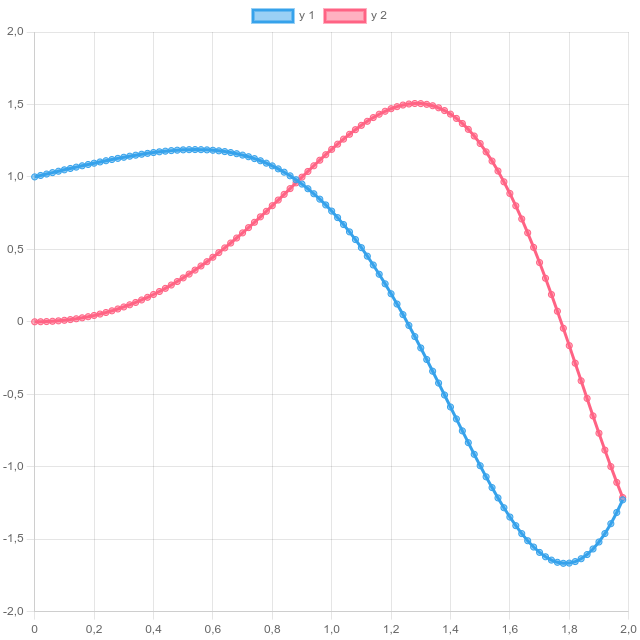
\includegraphics[width=0.31\linewidth]{pictures/testTaskResult.png}
    \captionsetup{labelformat=empty}
    \caption{Рис.1 --- График двух функций, полученных через метод Рунге - Кутты.}
\end{figure}

Решив таким образом систему, составим графики зависимости максимальной ошибки решения от шага $h^4$:
\begin{figure}[h]
    \centering
    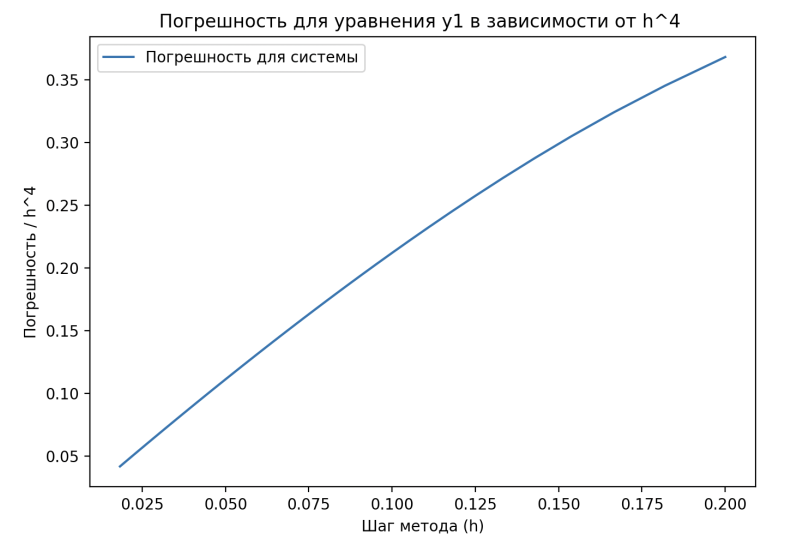
\includegraphics[width=0.5\linewidth]{pictures/testTask.png}
    \captionsetup{labelformat=empty}
    \caption{Рис.2 --- Зависимость точности решения от шага $h^4$.}
\end{figure}

Исходя из вида графиков, описывающих зависимость точности решения, можно сделать вывод
о зависимости точности решения от шага разбиения. 

\newpage


\section{Модель Вольтерра}
\hspace{0.5cm} Теперь мы можем, используя правило (4) решить систему (2). Выберем начальные условия
$X_0 = 3, Y_0 = 0.5$, начальное число жертв и хищников, соответственно. Исходя из вида системы, отметим, что
динамика популяции зависит от параметра $\sigma = \frac{c}{a}$ - отношения смертности хищников к приросту жертв.
Выбрав $\sigma = 1$, т.е. установив равное отношение прироста жертв к смертности хищников получим график 
описывающий размеры популяций жертв и хищников с течением времени (Рис.3). Размер популяции жертв 
в начальный момент превышает размер популяции хищников, из-за чего веротность встречи представителей двух
видов возрастает, хищник убивает жертву. С уменьшением количества жертв, количество встреч 
с хищниками убывает. Когда хищники не охотятся, их популяция начинает вымирать. Уменьшение популяции хищников уменьшает \\
вероятность встреч с жертвами, что для последних, при наличии бесконечного числа пищи 
является причиной резкого увеличения числа представителей вида. Резкое \\
увеличение числа жертв предполагает возрастание числа хищников. Система приходит в циклиеское, устойчивое состояние. 
На графике по горизонтали -- время, по вертикали -- популяция.
\begin{figure}[h]
    \centering
    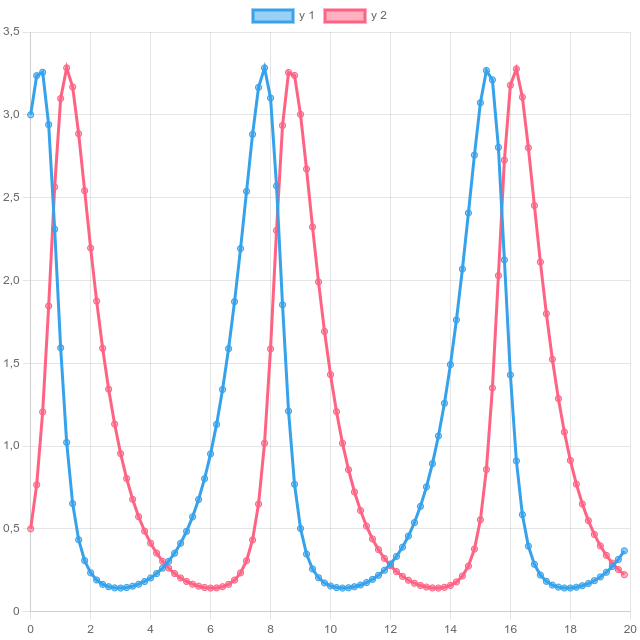
\includegraphics[width=0.5\linewidth]{pictures/task1.png}
    \captionsetup{labelformat=empty}
    \caption{Рис.3 --- Размер популяций жертв (синий) и хищников (красный) с течением времени.}
\end{figure}
\newpage

Теперь выберем $\sigma = 3$, что определит троекратное увеличение убыли хищников
к росту популяций жертв. Поведение популяций видов изменилось, численность популяций изменяется не так сильно,
однако, за тот же промежуток времени происходит большее число "колебаний" числа представителей вида (Рис.4).
\begin{figure}[h]
    \centering
    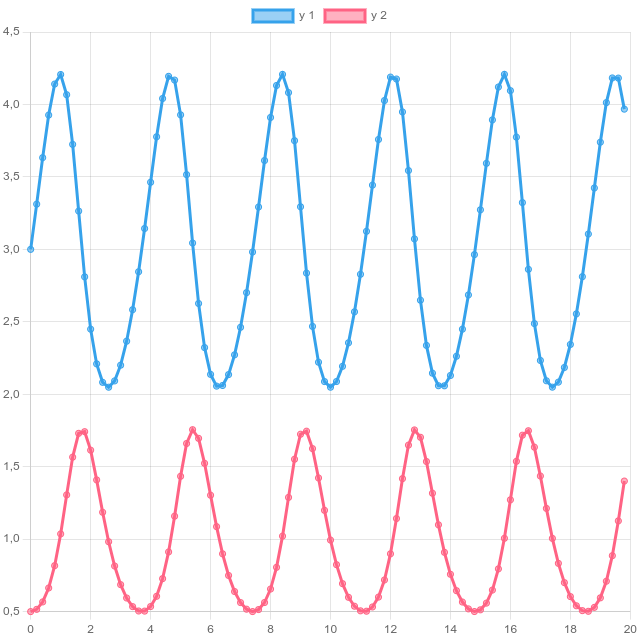
\includegraphics[width=0.5\linewidth]{pictures/task2.png}
    \captionsetup{labelformat=empty}
    \caption{Рис.4 --- Изменение популяций видов при $\sigma = 3$.}
\end{figure}

Применим те же параметры для системы с начальными условиями $X_0 = 1, Y_0 = 4$, что соответствует 
ситуации, когда в начальный момент число хищников в 4 раза превышает количество жертв.
Тенденция стаблизации системы сохраняется, однако при значении $\sigma = 3$ популяция 
хищников убывает сильнее из-за малого количества доступной изначально пищи и значения коэффициента.
\begin{figure}[h]
    \centering
    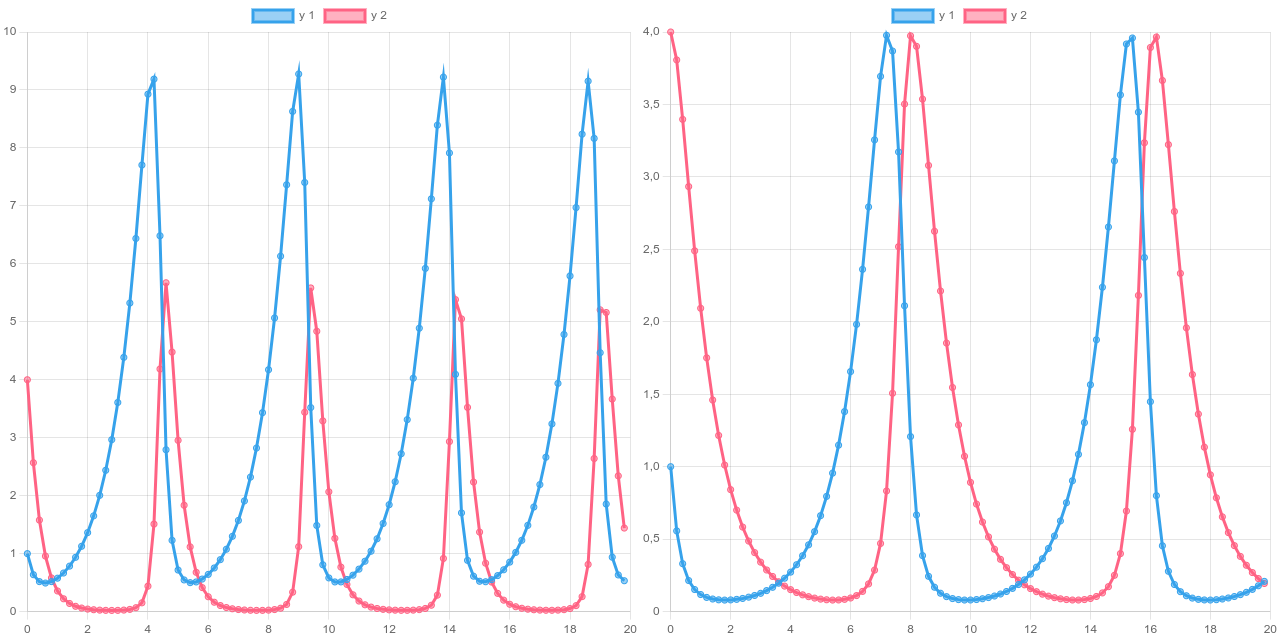
\includegraphics[width=0.8\linewidth]{pictures/task3.png}
    \captionsetup{labelformat=empty}
    \caption{Рис.5 --- Вид популяции при других начальных условиях.}
\end{figure}
\newpage

Представим графики в координатах $(X, Y)$ для двух расмотренных начальных условий (Рис. 6).
\begin{figure}[h]
    \centering
    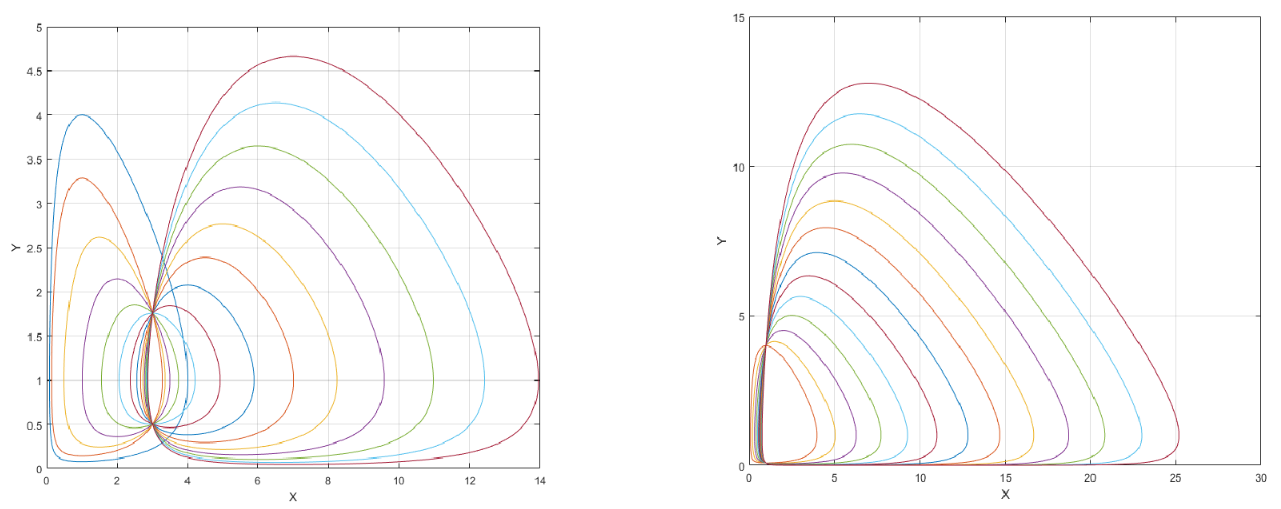
\includegraphics[width=1\linewidth]{pictures/task4.png}
    \captionsetup{labelformat=empty}
    \caption{Рис.6 --- Графики $(X, Y)$ в зависимости от параметра $\sigma$.}
\end{figure}

\newpage
\section{Заключение}
\hspace{0.5cm} Модель Вольтерра может быть использована для моделирования системы типа "Хищник--жертва".
Наблюдая за моделью можно выявить основные закономерности поведения популяций. В ходе работы были рассмотрены
модели с различными значениями начального размера популяций, коэффициентов определяющих отношение убыли 
одного вида к приросту другого. При выполнении задачи был использован метод Рунге--Кутты для решения систем 
дифференциалных уравнений. Метод позволяет решать уравнения с достаточной степенью точности, достаточной для 
корректного моделирования системы.
\newpage
\section{Cписок литературы}
\begin{enumerate}
    \item Глазырина Л.Л., Карчевский М.М. Численные методы: учебное пособие. — Казань: Казан.
    ун-т, 2012. — 122 
    \item Глазырина Л.Л.. Практикум по курсу «Численные методы». Решение
    систем линейных уравнений: учеб. пособие. — Казань: Изд-во Казан. ун-та, 2017. — 52 с.
    \item Дж. Ортега, У. Пул. Введение в численные методы решения дифференци-
    альных уравнений. — М.: Наука, 1986
    \item Самарский А.А., Гулин А.В. Численные методы. — М.: Наука, 1989.
    \item Бахвалов Н.С., Жидков Н.П., Кобельков Г.М. Численные методы. — М.:
    БИНОМ. Лаб. знаний, 2007.
    \item Глазырина Л. Л., Карчевский М. М. Введение в численные методы. —
    Казань, КГУ, 2012
\end{enumerate}
\newpage

\section{Листинг программы}
\lstinputlisting[language=C++]{../src/main.cpp}
\end{document}